% !TeX program = pdflatex
\documentclass[11pt,a4paper]{report}
\usepackage[margin=23mm]{geometry}
\usepackage[T5,T1]{fontenc}
\usepackage[utf8]{inputenc}
\usepackage[english,vietnamese]{babel}
\usepackage{lmodern,microtype,graphicx,booktabs,array,tabularx}
\usepackage{amsmath,amssymb,float,subcaption,xcolor,enumitem,fancyhdr,hyperref,placeins}
\graphicspath{{assets/}}
\hypersetup{colorlinks=true,linkcolor=blue!55!black,citecolor=blue!55!black,urlcolor=blue!55!black}
\setlength{\parindent}{0pt}\setlength{\parskip}{5pt}
\setcounter{secnumdepth}{3}\setcounter{tocdepth}{2}
\definecolor{navy}{RGB}{25,56,92}
\definecolor{passgreen}{RGB}{0,105,70}
\definecolor{failred}{RGB}{170,35,35}
\definecolor{warnorange}{RGB}{185,105,0}
\pagestyle{fancy}\fancyhf{}
\fancyhead[L]{\scriptsize\itshape Trường Đại học Khoa học Tự nhiên - Khoa Điện tử - Viễn thông}
\fancyhead[R]{\scriptsize\itshape Lê Phan Thanh Liêm}\fancyfoot[C]{\thepage}
\renewcommand{\headrulewidth}{0.4pt}
\fancypagestyle{plain}{\fancyhf{}\fancyhead[L]{\scriptsize\itshape Trường Đại học Khoa học Tự nhiên - Khoa Điện tử - Viễn thông}\fancyhead[R]{\scriptsize\itshape Lê Phan Thanh Liêm}\fancyfoot[C]{\thepage}\renewcommand{\headrulewidth}{0.4pt}}
\newcommand{\SI}[2]{\ensuremath{#1\,\mathrm{#2}}}
\newcommand{\si}[1]{\ensuremath{\mathrm{#1}}}
\newcommand{\SIrange}[3]{\ensuremath{#1\text{--}#2\,\mathrm{#3}}}
\newcommand{\ang}[1]{\ensuremath{#1^{\circ}}}
\newcommand{\micro}{\mu}\newcommand{\dd}{\mathrm d}\newcommand{\ohm}{\Omega}
\newcommand{\pass}{\textcolor{passgreen}{Đạt}}
\newcommand{\fail}{\textcolor{failred}{Chưa đạt}}
\newcommand{\pending}{\textcolor{warnorange}{Cần đo lại}}
\newcommand{\figwide}[3][0.96\textwidth]{\begin{figure}[H]\centering\includegraphics[width=#1]{#2}\caption{#3}\end{figure}}

\begin{document}
\begin{titlepage}\centering
\vspace*{7mm}
{\large\bfseries TRƯỜNG ĐẠI HỌC KHOA HỌC TỰ NHIÊN - ĐHQG TP.HCM\par}
\vspace{1.5mm}{\large\bfseries KHOA ĐIỆN TỬ - VIỄN THÔNG\par}
\vspace{7mm}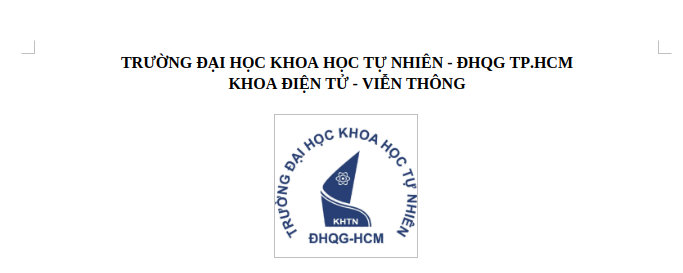
\includegraphics[width=31mm,trim=270 14 270 112,clip]{khtn_reference.png}\par
\vspace{10mm}{\Large\bfseries THIẾT KẾ VI MẠCH TƯƠNG TỰ\par}
\vspace{8mm}{\color{navy}\rule{\textwidth}{1.2pt}\par}\vspace{8mm}
{\Huge\bfseries THIẾT KẾ VÀ PHÂN TÍCH OP-AMP CMOS HAI TẦNG BÙ MILLER\par}
\vspace{7mm}{\Large Công nghệ GPDK090, Suppy \SI{1.2}{V}\par}
\vspace{8mm}{\color{navy}\rule{\textwidth}{1.2pt}\par}
\vfill
\begin{tabular}{rl}
\textbf{Sinh viên:}&Lê Phan Thanh Liêm\\
\textbf{Môi trường thiết kế:}&Cadence Virtuoso / Spectre\\
\textbf{Công nghệ:}&GPDK090 BSIM3\\
\textbf{Thời gian:}&Tháng 10 năm 2026
\end{tabular}
\vfill
\end{titlepage}

\pagenumbering{roman}
\chapter*{Tóm tắt}\addcontentsline{toc}{chapter}{Tóm tắt}
Báo cáo trình bày quá trình tính toán và kiểm chứng ở mức transistor của một op-amp CMOS hai tầng không có tầng đệm, sử dụng bù Miller. Mạch gồm cặp vi sai NMOS, tải tích cực gương dòng PMOS, nguồn dòng đuôi NMOS, tầng khuếch đại common-source PMOS và tải dòng NMOS ở ngõ ra. Nguồn nuôi danh định là \SI{1.2}{V}, tải ngoài \SI{10}{pF}, tụ Miller \SI{3.6}{pF} và dòng phân cực tham chiếu \SI{6.1}{\micro A}.

Thiết kế ban đầu hướng đến độ lợi DC ít nhất \SI{70}{dB}, unity frequency ít nhất \SI{3}{MHz}, slew rate \SI{5}{V/\micro s}, ICMR \SIrange{0.4}{0.9}{V} và phase margin xấp xỉ \ang{60}. Mô phỏng Spectre với điện trở nulling \SI{1.8}{k\ohm} cho độ lợi vòng hở tần số thấp \SI{74.05}{dB}, tần số unity khoảng \SI{3.802}{MHz} và phase margin khoảng \ang{62.13}. Khoảng common-mode đo được xấp xỉ \SIrange{0.313}{0.936}{V}. Đáp ứng follower với bước \SI{0.4}{V} có thời gian chuyển mức 10--90\% khoảng \SI{78.58}{ns} ở cạnh lên và \SI{89.40}{ns} ở cạnh xuống. CMRR, PSRR$^+$ và PSRR$^-$ tần số thấp lần lượt xấp xỉ \SI{73.60}{dB}, \SI{76.14}{dB} và \SI{87.48}{dB}; công suất tĩnh đo trực tiếp là \SI{153.249}{\micro W}.

\tableofcontents\clearpage\pagenumbering{arabic}

\chapter{Giới thiệu và yêu cầu thiết kế}
\section{Mục tiêu}
Mục tiêu là thiết kế, xác định kích thước và kiểm chứng một op-amp CMOS hai tầng nhỏ gọn trong công nghệ GPDK090. Quy trình bắt đầu từ tính toán giải tích, sau đó kiểm tra phân cực và bão hòa bằng DC operating point, đánh giá độ lợi và ổn định bằng AC, rồi đánh giá tốc độ tín hiệu lớn và thời gian xác lập bằng transient. Cơ sở lý thuyết và các quy trình thiết kế được tổng hợp trong phần tài liệu tham khảo cuối báo cáo.

\section{Kiến trúc}
\begin{itemize}[leftmargin=18mm]
\item M1--M2: cặp vi sai NMOS đối xứng;
\item M3--M4: tải tích cực gương dòng PMOS và chuyển đổi sang ngõ ra đơn đầu;
\item M5: nguồn dòng đuôi NMOS;
\item M6: tầng khuếch đại common-source PMOS;
\item M7: nguồn hút dòng NMOS ở tầng ngõ ra, dùng multiplicity $m=6$;
\item M8: NMOS mắc diode, chuyển $I_{BIAS}$ thành điện áp phân cực cho M5 và M7;
\item $C_C$: tụ Miller nối ngõ ra tầng một với ngõ ra op-amp.
\end{itemize}
\figwide[0.89\textwidth]{dc_operating.png}{Sơ đồ transistor cuối cùng với điện áp DC và kích thước linh kiện.}

\section{Khảo sát đặc tính NMOS và PMOS}
Trước khi tính kích thước cho op-amp, các transistor NMOS và PMOS của công nghệ
GPDK090 được khảo sát riêng bằng cấu hình mắc diode, tức là cực cổng nối với cực
máng. Khi đó $V_{DS}=V_{GS}$ đối với NMOS và $V_{SD}=V_{SG}$ đối với PMOS. Vì
điều kiện bão hòa luôn được thỏa mãn sau khi transistor dẫn, cấu hình này thuận
tiện để trích điện áp ngưỡng và tham số dẫn truyền dùng trong phần tính toán tay.

\begin{figure}[H]
\centering
\begin{subfigure}[t]{0.47\textwidth}
\centering
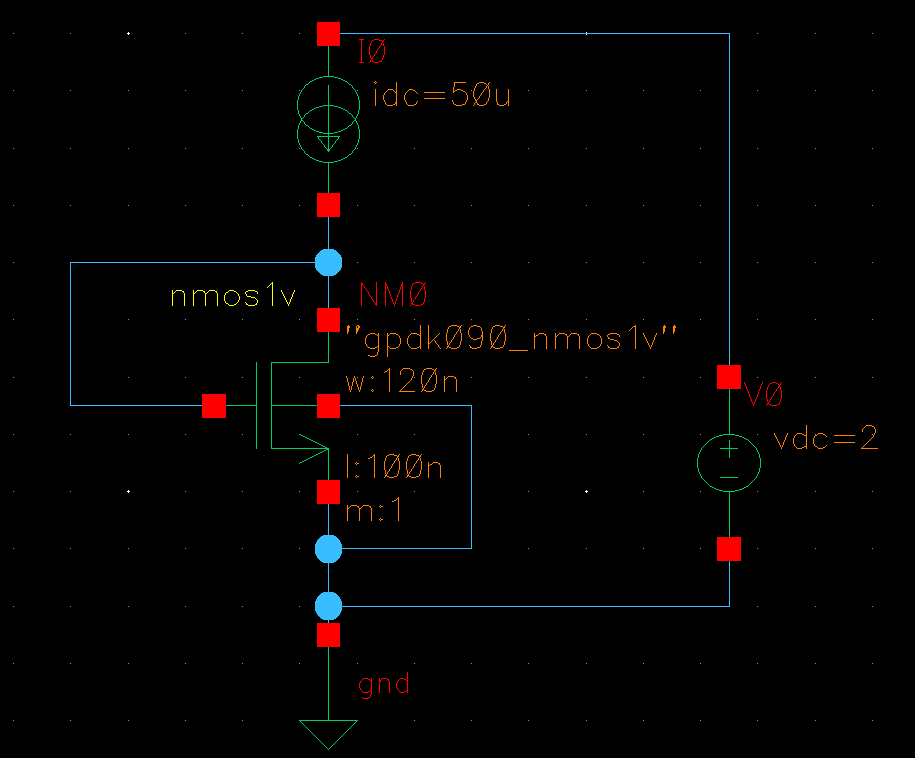
\includegraphics[width=\textwidth]{nmos_characterestic..png}
\caption{Mạch khảo sát NMOS mắc diode.}
\end{subfigure}\hfill
\begin{subfigure}[t]{0.47\textwidth}
\centering
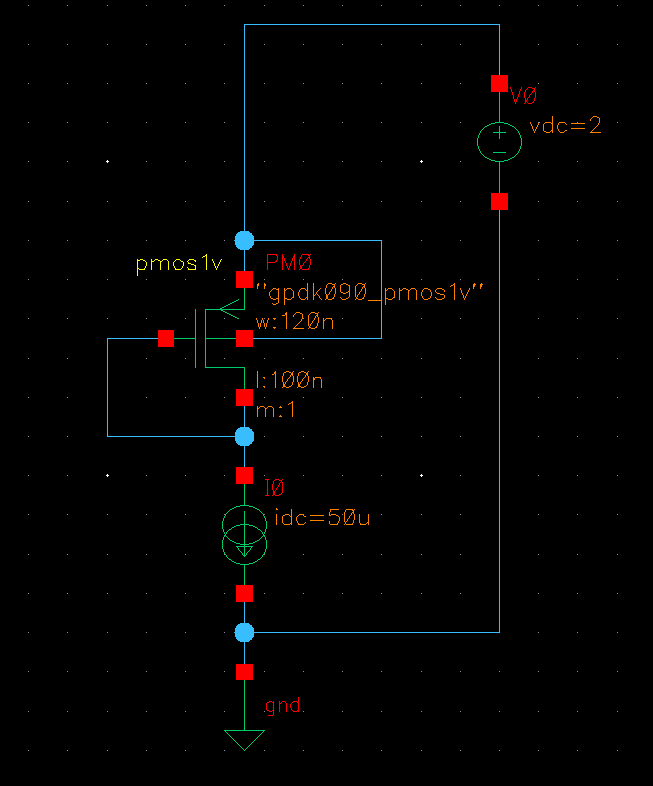
\includegraphics[width=\textwidth]{pmos_characterestic.png}
\caption{Mạch khảo sát PMOS mắc diode.}
\end{subfigure}
\caption{Các testbench dùng để khảo sát transistor GPDK090 với
$W=\SI{120}{nm}$, $L=\SI{100}{nm}$ và dòng thử $|I_D|=\SI{50}{\micro A}$.}
\label{fig:mos-characterization}
\end{figure}

Với mô hình square-law bỏ qua hiệu ứng điều biến chiều dài kênh, dòng bão hòa
được biểu diễn gần đúng bởi
\begin{align}
I_{D,n}&=\frac{1}{2}K_n'\frac{W}{L}(V_{GS}-V_{TN})^2,\\
|I_{D,p}|&=\frac{1}{2}K_p'\frac{W}{L}(V_{SG}-|V_{TP}|)^2.
\end{align}
Do đó, sau khi đọc $V_{GS}$ hoặc $V_{SG}$ và điện áp ngưỡng từ kết quả DC
operating point, tham số công nghệ được suy ra theo
\begin{equation}
K' = \frac{2|I_D|}{(W/L)V_{OV}^2},
\qquad V_{OV}=V_{GS}-V_{TN}\ \text{(NMOS)},\quad
V_{OV}=V_{SG}-|V_{TP}|\ \text{(PMOS)}.
\end{equation}
Điện áp ngưỡng của mô hình BSIM3 thay đổi nhẹ theo kích thước linh kiện và điểm
phân cực. Vì vậy, khi tính giới hạn ICMR, báo cáo sử dụng giá trị biên bất lợi
thay vì một giá trị ngưỡng danh định duy nhất. Các tham số được chốt cho phần
tính toán first-cut là
\begin{table}[H]\centering
\caption{Tham số NMOS và PMOS dùng trong tính toán giải tích.}
\begin{tabular}{lll}\toprule
Loại transistor&Tham số dẫn truyền&Điện áp ngưỡng sử dụng\\\midrule
NMOS&$K_n'=\SI{296.4}{\micro A/V^2}$&
$V_{TN,min}=\SI{0.151885}{V}$, $V_{TN,max}=\SI{0.186604}{V}$\\
PMOS&$K_p'=\SI{167.4}{\micro A/V^2}$&
$|V_{TP}|_{max}=\SI{0.149135}{V}$\\\bottomrule
\end{tabular}
\end{table}
Các giá trị trên chỉ được dùng cho mô hình square-law trong bước tính tay;
mọi mô phỏng Spectre phía sau vẫn sử dụng đầy đủ mô hình BSIM3 của GPDK090.

\section{Thông số mục tiêu và hằng số thiết kế}
\begin{table}[H]\centering\caption{Yêu cầu thiết kế và điều kiện cố định.}
\begin{tabularx}{\textwidth}{>{\bfseries}l >{\raggedright\arraybackslash}X l}\toprule
Thông số&Giá trị mục tiêu / lựa chọn&Ký hiệu\\\midrule
Nguồn nuôi&$V_{DD}=\SI{1.2}{V}$, $V_{SS}=\SI{0}{V}$&$V_{DD},V_{SS}$\\
Độ lợi DC vòng hở&ít nhất \SI{70}{dB}&$A_0$\\
Unity frequency&ít nhất \SI{3}{MHz}&$f_u$\\
Phase margin&xấp xỉ \ang{60} hoặc lớn hơn&PM\\
Tụ tải&\SI{10}{pF}&$C_L$\\
Tụ Miller&\SI{3.6}{pF}&$C_C$\\
Slew rate&\SI{5}{V/\micro s}&SR\\
Thời gian xác lập 1\%&không quá \SI{1}{\micro s} cho bước \SI{0.4}{V}&$t_s$\\
ICMR&\SIrange{0.4}{0.9}{V}&ICMR\\
Dòng tham chiếu&\SI{6.1}{\micro A}&$I_{BIAS}$\\
Tham số công nghệ&$K_n'=\SI{296.4}{\micro A/V^2}$, $K_p'=\SI{167.4}{\micro A/V^2}$&$K_n',K_p'$\\\bottomrule
\end{tabularx}\end{table}

\chapter{Thiết kế giải tích first-cut}
\section{Các quan hệ thiết kế}
Phần này thiết lập các công thức dùng cho quá trình sizing từ mô hình tín hiệu
nhỏ của op-amp hai tầng bù Miller. Mô hình tương đương được trình bày trong
Hình~\ref{fig:two-stage-small-signal}.

\begin{figure}[H]
\centering
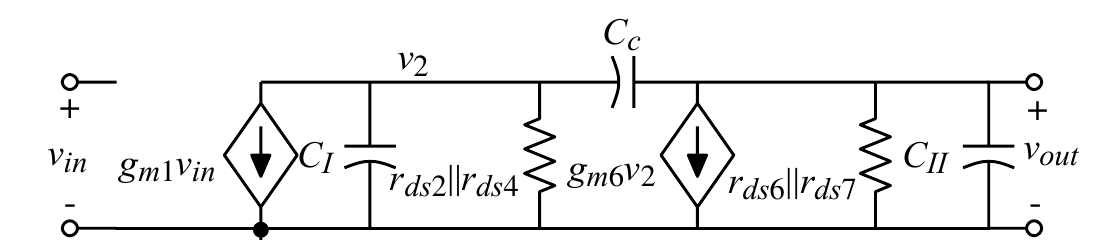
\includegraphics[width=0.96\textwidth]{two_stage_small_signal_model.png}
\caption{Mô hình tín hiệu nhỏ rút gọn của op-amp hai tầng bù Miller. Nút tầng
một được ký hiệu là $v_2$ trong hình; trong phần chứng minh phía dưới nút này
được đổi tên thành $v_1$ để thống nhất với ký hiệu của báo cáo.}
\label{fig:two-stage-small-signal}
\end{figure}

Đặt
\begin{equation}
R_I=r_{ds2}\parallel r_{ds4},\qquad
R_{II}=r_{ds6}\parallel r_{ds7},
\end{equation}
trong đó $R_I$ là điện trở ngõ ra tầng vi sai và $R_{II}$ là điện trở ngõ ra
tầng common-source. Điện dung tương đương tại hai nút lần lượt là $C_I$ và
$C_{II}$; với tải ngoài chiếm ưu thế, $C_{II}\simeq C_L$. Tụ bù $C_C$ nối giữa
hai nút này.

Về mặt vật lý, $R_I$ và $C_I$ mô tả nút có trở kháng cao ở ngõ ra tầng một,
còn $R_{II}$ và $C_{II}$ mô tả nút ngõ ra của toàn op-amp. Nếu không có bù,
hai nút trở kháng cao này tạo ra hai cực có thể nằm khá gần nhau. Khi vòng hồi
tiếp đi qua hai cực trước khi độ lợi giảm xuống 1, tổng trễ pha tiến gần
\ang{180} và mạch dễ dao động. Vai trò của $C_C$ là chủ động tách hai cực:
kéo một cực xuống thấp để trở thành cực trội và đẩy cực còn lại lên cao hơn.

\subsection{Độ lợi DC của hai tầng}
Ở tần số thấp, $C_C$ hở mạch. Tầng thứ nhất biến dòng tín hiệu nhỏ của cặp vi
sai thành điện áp tại nút $v_1$, còn tầng thứ hai M6 khuếch đại đảo điện áp này.
Bỏ qua dấu pha khi chỉ xét độ lớn,
\begin{align}
A_{v1}&\simeq g_{m1}R_I
=\frac{g_{m1}}{g_{ds2}+g_{ds4}},\\
A_{v2}&\simeq g_{m6}R_{II}
=\frac{g_{m6}}{g_{ds6}+g_{ds7}},\\
A_0&\simeq A_{v1}A_{v2}
=g_{m1}g_{m6}R_IR_{II}.
\end{align}
Do M1 và M2 đối xứng, $g_{m1}=g_{m2}$ tại điểm phân cực; vì vậy ký hiệu
$g_{m1}$ bên dưới cũng chính là transconductance của mỗi transistor ngõ vào.

Có thể hiểu từng thừa số trong $A_0$ theo chuỗi biến đổi
\begin{equation}
v_{in}\ \xrightarrow{\ g_{m1}\ }\ i_1
\ \xrightarrow{\ R_I\ }\ v_1
\ \xrightarrow{\ g_{m6}\ }\ i_o
\ \xrightarrow{\ R_{II}\ }\ v_o.
\end{equation}
Do đó, muốn tăng độ lợi DC có thể tăng $g_m$ hoặc tăng $r_{ds}$. Tuy nhiên tăng
$g_m$ thường cần thêm dòng hoặc tăng kích thước transistor, còn tăng $r_{ds}$
thường cần tăng chiều dài kênh. Công thức trên vì thế không chỉ dùng để tính
gain mà còn cho thấy trực tiếp các đánh đổi về công suất, diện tích và tốc độ.

\subsection{Hàm truyền của mạch bù Miller}
Viết KCL tại nút $v_1$ và $v_o$ của mô hình tín hiệu nhỏ trong
Hình~\ref{fig:two-stage-small-signal} thu được
\begin{align}
-g_{m1}v_{in}
&=\left[G_I+s(C_I+C_C)\right]v_1-sC_Cv_o,\\
0&=(g_{m6}-sC_C)v_1+\left[G_{II}+s(C_{II}+C_C)\right]v_o,
\end{align}
với $G_I=1/R_I$ và $G_{II}=1/R_{II}$. Giải hệ hai phương trình cho
$A(s)=v_o/v_{in}$ cho kết quả
\begin{equation}
A(s)=\frac{g_{m1}(g_{m6}-sC_C)}
{G_IG_{II}+a_1s+a_2s^2},
\end{equation}
trong đó
\begin{align}
a_1&=G_{II}(C_I+C_C)+G_I(C_{II}+C_C)+g_{m6}C_C,\\
a_2&=C_IC_{II}+C_CC_I+C_CC_{II}.
\end{align}
Chuẩn hóa mẫu số theo $G_IG_{II}$ cho dạng dễ nhận biết hơn:
\begin{align}
A(s)&=A_0\frac{1-sC_C/g_{m6}}{1+b_1s+b_2s^2},\\
b_1&=R_I(C_I+C_C)+R_{II}(C_{II}+C_C)
+g_{m6}R_IR_{II}C_C,\\
b_2&=R_IR_{II}(C_IC_{II}+C_CC_I+C_CC_{II}).
\end{align}

Hai phương trình KCL trên có thể đọc theo từng thành phần như sau. Trong phương
trình thứ nhất, $g_{m1}v_{in}$ là dòng tín hiệu do cặp vi sai tạo ra;
$G_Iv_1$ là dòng qua điện trở ngõ ra tầng một; $sC_Iv_1$ là dòng qua điện dung
ký sinh tại nút này; còn $sC_C(v_1-v_o)$ là dòng đi qua tụ Miller. Trong phương
trình thứ hai, $g_{m6}v_1$ là dòng do M6 tạo ra, $G_{II}v_o+sC_{II}v_o$ là dòng
tại nút ngõ ra và $sC_C(v_o-v_1)$ vẫn là dòng qua cùng tụ bù nhưng nhìn từ phía
còn lại. Viết rõ các dòng như vậy giúp kiểm tra dấu trước khi giải hệ, đặc biệt
vì sai dấu của nhánh $C_C$ sẽ làm zero xuất hiện ở sai nửa mặt phẳng.

Sau khi chuẩn hóa, tử số quyết định zero còn mẫu số quyết định các pole. Hệ số
$b_1$ là tổng các hằng số thời gian bậc nhất. Trong đó,
$g_{m6}R_IR_{II}C_C$ là thành phần Miller và thường lớn nhất. Hệ số $b_2$ chứa
tích của hai điện trở nút với các tích điện dung, nên quyết định sự tương tác
giữa hai cực. Đây là lý do ta không thể chỉ nhìn riêng $R_IC_I$ và
$R_{II}C_{II}$ sau khi đã nối $C_C$ giữa hai nút.

\subsection{Zero RHP, cực trội và cực thứ hai}
Tử số bằng không tại
\begin{equation}
z_{RHP}=+\frac{g_{m6}}{C_C}.
\end{equation}
Dấu dương cho biết đây là zero ở nửa mặt phẳng phải: zero này làm tăng biên độ
nhưng đồng thời tạo trễ pha, do đó bất lợi cho ổn định. Khi hiệu ứng Miller chiếm
ưu thế,
$g_{m6}R_IR_{II}C_C$ lớn hơn các hằng số thời gian còn lại. Nếu hai cực tách xa
nhau, $|p_2|\gg|p_1|$, các nghiệm của mẫu số xấp xỉ
\begin{align}
p_1&\simeq-\frac{1}{g_{m6}R_IR_{II}C_C}
=-\frac{(g_{ds2}+g_{ds4})(g_{ds6}+g_{ds7})}{g_{m6}C_C},\\
p_2&\simeq-\frac{g_{m6}C_C}
{C_IC_{II}+C_CC_I+C_CC_{II}}
\simeq-\frac{g_{m6}}{C_{II}}
\simeq-\frac{g_{m6}}{C_L}.
\end{align}
$p_1$ là cực trội do hiệu ứng Miller, còn $p_2$ chủ yếu là cực tại ngõ ra.
Xấp xỉ cuối của $p_2$ đòi hỏi $C_{II}>C_C>C_I$ và $C_{II}\simeq C_L$.

Nguồn gốc của zero RHP có thể giải thích bằng đường truyền thẳng qua $C_C$.
Ở tần số đủ cao, tụ Miller truyền trực tiếp biến thiên tại $v_1$ sang ngõ ra.
Dòng này có chiều làm ngõ ra thay đổi ngược với tác dụng mong muốn của tầng M6,
vì vậy nó tạo một zero không minimum-phase. Một zero LHP cũng làm tăng biên độ
nhưng tạo sớm pha; trái lại zero RHP tạo thêm trễ pha. Do đó chỉ kiểm tra đồ thị
biên độ mà không kiểm tra phase có thể dẫn tới kết luận sai về độ ổn định.

\subsubsection{Ảnh hưởng của điện trở nulling $R_z$}
Khi mắc điện trở $R_z$ nối tiếp với tụ Miller, trở kháng của nhánh bù trở thành
\begin{equation}
Z_C(s)=R_z+\frac{1}{sC_C}.
\end{equation}
Điện trở này làm thay đổi dòng truyền thẳng qua nhánh bù nhưng gần như không làm
mất tác dụng Miller của $C_C$ ở vùng tần số thấp. Trong xấp xỉ tín hiệu nhỏ,
vị trí zero được viết
\begin{equation}
\boxed{z=\frac{1}{C_C\left(1/g_{m6}-R_z\right)}}.
\end{equation}
Biểu thức này cho ba trường hợp quan trọng:
\begin{enumerate}[leftmargin=13mm]
\item Nếu $R_z=0$, thu lại $z=+g_{m6}/C_C$: zero nằm ở nửa mặt phẳng phải và
gây thêm trễ pha.
\item Nếu $R_z=1/g_{m6}$, mẫu của biểu thức tiến tới zero và zero được đẩy ra
vô cùng. Khi đó đường truyền thẳng qua $C_C$ bị triệt tiêu xấp xỉ, nên $R_z$
được gọi là điện trở \emph{nulling}.
\item Nếu $R_z>1/g_{m6}$, zero đổi dấu và chuyển sang nửa mặt phẳng trái:
\begin{equation}
z_{LHP}=-\frac{1}{C_C\left(R_z-1/g_{m6}\right)}.
\end{equation}
Zero LHP tạo sớm pha và có thể hỗ trợ phase margin, nhưng nếu nằm quá gần
unity frequency thì nó cũng làm thay đổi mạnh đáp ứng biên độ.
\end{enumerate}

Tại operating point của mạch, $g_{m6}\approx\SI{551}{\micro S}$ nên
\begin{equation}
\frac{1}{g_{m6}}\approx\SI{1.815}{k\ohm}.
\end{equation}
Giá trị sử dụng $R_z=\SI{1.8}{k\ohm}$ rất gần giá trị này. Nếu dùng trực tiếp
các số operating point và $C_C=\SI{3.6}{pF}$, zero còn lại được ước lượng ở
vùng vài gigahertz, xa hơn nhiều so với
$f_u\approx\SI{3.802}{MHz}$. Vì vậy đóng góp trễ pha của zero tại unity
frequency trở nên rất nhỏ; kết quả AC cho phase margin \ang{62.13} phù hợp với
cơ chế này.

Điều kiện $R_z=1/g_{m6}$ chỉ là xấp xỉ vì $g_{m6}$ thay đổi theo điểm phân cực,
process, điện áp và nhiệt độ. Do đó không nên kết luận ổn định chỉ từ phép tính
$R_z$; vị trí pole--zero và phase margin cuối cùng vẫn phải được kiểm tra bằng
mô phỏng AC, PVT và mô phỏng hậu layout.

Để thấy cách thu được hai xấp xỉ pole, viết mẫu số thành
$(1-s/p_1)(1-s/p_2)$. Khi $|p_2|\gg|p_1|$, hệ số bậc nhất gần như bằng
$-1/p_1$, còn tỷ số giữa hệ số bậc nhất và bậc hai gần bằng $-p_2$. Vì thành
phần Miller chiếm ưu thế trong $b_1$, ta có
$p_1\simeq-1/(g_{m6}R_IR_{II}C_C)$. Lấy $b_1/b_2$ và dùng
$C_{II}>C_C>C_I$ cho $p_2\simeq-g_{m6}/C_{II}$. Các bước này chỉ hợp lệ khi
hai pole thực sự tách xa; nếu không, phải dùng nghiệm đầy đủ của phương trình
bậc hai hoặc đọc trực tiếp từ mô phỏng AC.

\subsection{Unity-gain bandwidth và điều kiện phase margin}
Vì $|p_1|$ là cực trội,
\begin{equation}
\omega_u\simeq A_0|p_1|
=\frac{g_{m1}}{C_C}.
\end{equation}
Đại lượng $\omega_u$ ở trên có đơn vị rad/s. Trong báo cáo, GBW được cho theo
hertz nên phải đổi đơn vị:
\begin{equation}
\boxed{GBW=f_u\simeq\frac{g_{m1}}{2\pi C_C}}.
\end{equation}
Kết quả trên có ý nghĩa thiết kế rất rõ: sau khi $C_C$ đã được chọn từ yêu cầu
ổn định và slew rate, GBW gần như được quyết định trực tiếp bởi $g_{m1}$. Vì
vậy ta có thể tính ngược $g_{m1}=2\pi\,GBW\,C_C$, rồi từ $g_{m1}$ và dòng phân
cực suy ra kích thước M1--M2. Điện trở ngõ ra không xuất hiện trong biểu thức
GBW vì $R_I$ và $R_{II}$ đã triệt tiêu khi nhân $A_0$ với $|p_1|$; chúng vẫn
ảnh hưởng mạnh đến độ lợi DC nhưng không chi phối unity frequency trong xấp xỉ
cực trội này.

Tại $\omega=\omega_u$, cực trội đã tạo gần \ang{90} trễ pha. Nếu đặt zero RHP
đủ xa, $z_{RHP}\ge10\omega_u$, đóng góp pha của zero không quá
$\tan^{-1}(0.1)\simeq\ang{5.7}$. Với phase margin mục tiêu \ang{60}, cực thứ
hai phải thỏa
\begin{equation}
\tan^{-1}\!\left(\frac{\omega_u}{|p_2|}\right)
\lesssim\ang{24.3}
\quad\Longrightarrow\quad
|p_2|\gtrsim2.2\omega_u.
\end{equation}
Con số $2.2$ không phải một hệ số kinh nghiệm tùy ý. Ngân sách pha còn lại cho
cực thứ hai là khoảng
$\ang{180}-\ang{60}-\ang{90}-\ang{5.7}=\ang{24.3}$; do đó
$\omega_u/|p_2|\le\tan(\ang{24.3})\simeq0.455$, hay
$|p_2|/\omega_u\gtrsim2.2$. Nếu zero RHP nằm gần hơn $10\omega_u$, nó tiêu tốn
nhiều ngân sách pha hơn và yêu cầu $p_2\ge2.2\omega_u$ không còn đủ để bảo đảm
phase margin \ang{60}.
Thay các xấp xỉ của $p_2$ và $\omega_u$ vào biểu thức trên:
\begin{equation}
\boxed{g_{m6}\gtrsim2.2g_{m1}\frac{C_L}{C_C}}.
\end{equation}
Đồng thời, điều kiện đưa zero RHP ra ít nhất mười lần unity frequency là
\begin{equation}
\frac{g_{m6}}{C_C}\ge10\frac{g_{m1}}{C_C}
\quad\Longrightarrow\quad
\boxed{g_{m6}\ge10g_{m1}}.
\end{equation}
Nếu chọn $g_{m6}\simeq10g_{m1}$ để vừa thỏa điều kiện zero, hai điều kiện trên
cho
\begin{equation}
10g_{m1}\gtrsim2.2g_{m1}\frac{C_L}{C_C}
\quad\Longrightarrow\quad
\boxed{C_C\gtrsim0.22C_L}.
\end{equation}
Như vậy hệ số $2.2$ không tự nó bảo đảm ảnh hưởng của zero RHP là nhỏ; cần kiểm
tra đồng thời cả $p_2$ và $z_{RHP}$. Điều kiện trên được trình bày cho trường
hợp bù Miller thuần túy; mạch cuối cùng dùng điện trở nulling nối tiếp $C_C$ để
đẩy zero RHP ra xa, thay vì buộc $g_{m6}$ phải tăng đến $10g_{m1}$.

Trình tự sử dụng các điều kiện trong quá trình thiết kế nên là: trước hết chọn
$C_C$ đủ lớn so với $C_L$; tiếp theo tính $g_{m1}$ từ GBW; sau đó chọn $g_{m6}$
đủ lớn để đẩy $p_2$ lên cao; cuối cùng kiểm tra vị trí zero RHP. Nếu yêu cầu
$g_{m6}\ge10g_{m1}$ làm dòng tầng hai quá lớn, điện trở nulling là cách tách bài
toán zero khỏi yêu cầu tăng $g_{m6}$, nhờ đó có thể giảm đánh đổi công suất.

\subsection{Slew rate và giới hạn của công thức}
Slew rate là hiện tượng tín hiệu lớn, xảy ra khi dòng nạp hoặc xả tụ bị giới hạn.
Từ $i_C=C\,\dd v_C/\dd t$, hai chiều chuyển mức của op-amp hai tầng được viết:
\begin{align}
SR_+&=\min\!\left(\frac{I_5}{C_C},
\frac{I_6-I_5-I_7}{C_L}\right),\\
SR_-&=\min\!\left(\frac{I_5}{C_C},
\frac{I_7-I_5}{C_L}\right).
\end{align}
Khi bước điện áp vi sai đủ lớn, một transistor của cặp M1--M2 gần như nhận toàn
bộ dòng đuôi còn transistor kia gần như tắt. Lúc này tầng vào không còn làm việc
trong miền tín hiệu nhỏ và dòng qua $C_C$ bị chặn ở mức xấp xỉ $I_5$. Tốc độ
thay đổi điện áp trên tụ vì thế không thể vượt quá $I_5/C_C$. Ở ngõ ra, M6 và
M7 đồng thời phải nạp hoặc xả $C_L$; lượng dòng ròng còn lại ở hai chiều được
biểu diễn bởi số hạng thứ hai trong mỗi phép lấy $\min$. Tốc độ toàn mạch luôn
do nhánh chậm hơn quyết định.
Nếu dòng khả dụng của tầng ngõ ra đủ lớn so với $I_5$ và $C_L$ không quá lớn,
nhánh giới hạn là dòng đuôi nạp/xả tụ Miller, do đó
\begin{equation}
\boxed{SR\simeq\frac{I_5}{C_C}}.
\end{equation}
Ngược lại, khi tải lớn hoặc M6/M7 không cung cấp đủ dòng, một trong các số hạng
liên quan đến $C_L$ sẽ nhỏ hơn và công thức $I_5/C_C$ sẽ dự đoán SR quá lạc
quan. Vì vậy cả $SR_+$ và $SR_-$ phải được kiểm tra bằng mô phỏng transient.

Cũng cần phân biệt slew rate với GBW. GBW là thông số tín hiệu nhỏ và được xác
định khi transistor dao động quanh điểm phân cực; slew rate là giới hạn tín hiệu
lớn khi dòng đã bão hòa ở một giá trị cực đại. Một op-amp có GBW cao vẫn có thể
có slew rate thấp nếu dòng nạp/xả tụ nhỏ. Ngược lại, tăng dòng để cải thiện slew
rate không tự động bảo đảm phase margin nếu vị trí $p_2$ và zero RHP chưa phù
hợp.

Các quan hệ trên là xấp xỉ first-cut, dựa trên mô hình tín hiệu nhỏ, các cực tách
xa nhau và bỏ qua một số điện dung ký sinh. Kết quả thiết kế cuối cùng vẫn phải
được kiểm tra bằng operating point, AC và transient với mô hình BSIM3 đầy đủ.

\section{Tụ bù và dòng đuôi}
Điều kiện $C_C>0.22C_L$ cho $C_C>\SI{2.2}{pF}$. Chọn \SI{3.6}{pF} để tăng phân tách pole. Từ slew rate,
\begin{equation}I_5=SR\,C_C=(\SI{5}{V/\micro s})(\SI{3.6}{pF})=\boxed{\SI{18}{\micro A}}.\end{equation}

\section{Cặp vi sai và gương PMOS}
Mặc dù yêu cầu tối thiểu của unity frequency là \SI{3}{MHz}, bước sizing
first-cut chọn mốc thiết kế \SI{5}{MHz} để tạo dự phòng cho điện dung ký sinh
và sai khác giữa mô hình square-law với BSIM3:
\begin{equation}g_{m1}=2\pi(\SI{5}{MHz})(\SI{3.6}{pF})=\boxed{\SI{113.10}{\micro S}}.\end{equation}
Tại $V_{in,max}=\SI{0.9}{V}$,
\begin{align}V_{OV3}&=V_{DD}-V_{in,max}-|V_{TP}|_{max}+V_{TN,min}=\SI{0.30275}{V},\\
S_3=S_4&=\frac{I_5}{K_p'V_{OV3}^2}=\boxed{1.173},\\
S_1=S_2&=\frac{g_{m1}^2}{K_n'I_5}=\boxed{2.397}.
\end{align}

\section{Nguồn dòng đuôi M5}
\begin{equation}V_{OV1}=\sqrt{\frac{I_5}{K_n'S_1}}=\SI{0.15915}{V}.\end{equation}
Dùng $V_{in,min}=\SI{0.45}{V}$ để giữ dự phòng bão hòa:
\begin{align}V_{DS5,sat}&=0.45-0.15915-0.186604=\SI{0.10424}{V},\\
S_5&=\frac{2I_5}{K_n'V_{DS5,sat}^2}=\boxed{11.178}.
\end{align}
Kết quả square-law dự đoán biên ICMR thấp gần \SI{0.45}{V}; yêu cầu \SI{0.4}{V} phải được xác minh bằng mô hình transistor.

\section{Tầng thứ hai M6 và M7}
\begin{align}g_{m4}&=I_5/V_{OV3}=\SI{59.45}{\micro S},\\
g_{m6}&=2.2(\SI{113.10}{\micro S})\frac{10}{3.6}=\SI{691.15}{\micro S},\\
S_6&=(g_{m6}/g_{m4})S_4=13.637,\\
I_6&=g_{m6}^2/(2K_p'S_6)=\SI{104.62}{\micro A},\\
S_7&=(I_6/I_5)S_5=64.968.
\end{align}
Giá trị $g_{m6}$ trên được chọn theo điều kiện
$|p_2|\gtrsim2.2\omega_u$. Tuy nhiên,
$10g_{m1}=\SI{1.131}{mS}>g_{m6}=\SI{0.691}{mS}$, nên thiết kế first-cut này
chưa tự bảo đảm $z_{RHP}\ge10\omega_u$ nếu chỉ dùng tụ Miller. Vì vậy mạch cuối
cùng thêm điện trở nulling $R_z=\SI{1.8}{k\ohm}$ nối tiếp với $C_C$ để kiểm soát
zero. Kết quả AC sau khi thêm $R_z$ cho phase margin khoảng \ang{62.13}, đạt
mục tiêu \ang{60} mà không cần tăng mạnh dòng tầng hai.

\section{M8 và kích thước cuối}
Do M8 và M5 cùng $V_{GS}$,
\begin{equation}S_8=S_5\frac{I_{BIAS}}{I_5}=11.178\frac{6.1}{18}=\boxed{3.788}.\end{equation}
\begin{table}[H]\centering\caption{Kích thước tính toán và kích thước sử dụng.}
\begin{tabular}{cccccc}\toprule
MOS&$S$ tính toán&$W$ first-cut&$W$ cuối&$L$ cuối&$m$\\
& &(\si{\micro m})&(\si{\micro m})&(\si{\micro m})&\\\midrule
M1,M2&2.397&2.59&2.60&1.08&1\\
M3,M4&1.173&1.27&1.26&1.08&1\\
M5&11.178&16.10&16.10&1.44&1\\
M6&13.637&19.64&19.63&1.44&1\\
M7&64.968 hiệu dụng&15.59/finger&15.30&1.44&6\\
M8&3.788&5.45&5.45&1.44&1\\\bottomrule
\end{tabular}\end{table}
Ước lượng công suất tĩnh:
\begin{equation}P_{DC}\approx1.2(18+104.62+6.1)\,\si{\micro A}=\boxed{\SI{154.5}{\micro W}}.\end{equation}

\chapter{Phân tích DC}
\section{Kiểm tra operating point}
Operating point được đánh giá tại $V_{IN+}=V_{IN-}=\SI{0.6}{V}$ với $C_L=\SI{10}{pF}$. Sơ đồ cho $V_{OUT}\approx\SI{0.598}{V}$ và mọi transistor đều ở region 2.
\figwide[0.84\textwidth]{dc_operating.png}{Operating point tại $V_{IN+}=V_{IN-}=\SI{0.6}{V}$.}
Các nút quan trọng: nguồn chung M1--M2 khoảng \SI{0.2338}{V}; hai nút drain tầng một khoảng \SI{0.6929}{V} và \SI{0.7006}{V}; nút bias khoảng \SI{0.273}{V}; M6 có $V_{SD6}\approx\SI{0.602}{V}$ và M7 có $V_{DS7}\approx\SI{0.598}{V}$. Ngõ ra chỉ thấp hơn giữa nguồn khoảng \SI{2.1}{mV}.
\figwide[0.98\textwidth]{op_table.jpeg}{Các đại lượng operating point M1--M8 từ Spectre.}
\begin{table}[H]\centering\caption{Operating point danh định.}
\begin{tabular}{crrrcc}\toprule
MOS&$I_D$&$g_m$&$g_{ds}$&Region&$|V_{DS}|$\\\midrule
M1&\SI{8.893}{\micro A}&\SI{101.43}{\micro S}&\SI{6.26}{nS}&2&\SI{0.959}{V}\\
M2&\SI{8.898}{\micro A}&\SI{101.48}{\micro S}&\SI{6.21}{nS}&2&\SI{0.487}{V}\\
M3&\SI{8.892}{\micro A}&\SI{46.48}{\micro S}&\SI{467.24}{nS}&2&\SI{0.507}{V}\\
M4&\SI{8.83}{\micro A}&\SI{46.45}{\micro S}&\SI{480.29}{nS}&2&\SI{0.499}{V}\\
M5&\SI{17.79}{\micro A}&\SI{282.5}{\micro S}&\SI{1.73}{\micro S}&2&\SI{0.234}{V}\\
M6&\SI{103.82}{\micro A}&\SI{551.0}{\micro S}&\SI{3.65}{\micro S}&2&\SI{0.602}{V}\\
M7&\SI{103.82}{\micro A}&\SI{1.60}{mS}&\SI{5.78}{\micro S}&2&\SI{0.598}{V}\\
M8&\SI{6.09}{\micro A}&\SI{96.49}{\micro S}&\SI{0.464}{\micro S}&2&\SI{0.273}{V}\\\bottomrule
\end{tabular}\end{table}

\section{Công suất tĩnh}
Dòng lấy từ nguồn \SI{1.2}{V} được đo trực tiếp tại nguồn áp $V_3$ trong phép
phân tích DC operating point. Cadence trả về $i(V_3)=\SI{-127.707}{\micro A}$
và công suất của nguồn là \SI{-153.249}{\micro W}. Dấu âm xuất hiện do quy ước
chiều dòng và công suất của nguồn áp: nguồn đang cấp năng lượng cho mạch. Vì
vậy công suất mạch tiêu thụ được lấy theo trị tuyệt đối:
\begin{equation}
P_{DC}=V_{DD}|I_{DD}|=(\SI{1.2}{V})(\SI{127.707}{\micro A})
=\boxed{\SI{153.249}{\micro W}}.
\end{equation}
Giá trị đo chỉ thấp hơn ước lượng first-cut \SI{154.5}{\micro W} khoảng
\SI{1.251}{\micro W}, tương đương $0.81\%$; do đó phép ước lượng từ
các dòng nhánh phù hợp tốt với mô phỏng BSIM3.

\section{Ước lượng gain từ operating point}
\begin{align}A_{v1}&\approx\frac{101.475\,\si{\micro S}}{6.21\,\si{nS}+480.291\,\si{nS}}=208.6\;(\SI{46.39}{dB}),\\
A_{v2}&\approx\frac{550.997\,\si{\micro S}}{3.649\,\si{\micro S}+5.78\,\si{\micro S}}=58.44\;(\SI{35.33}{dB}),\\
A_{0,OP}&\approx1.219\times10^4\;(\SI{81.72}{dB}).
\end{align}
Mô phỏng AC đầy đủ cho \SI{74.05}{dB}; sai lệch \SI{7.7}{dB} phản ánh tải liên tầng, body transconductance, phần tử nội tại theo tần số và trở kháng hữu hạn của mạng bias.

\section{ICMR}
Để đo input common-mode range, op-amp được mắc voltage follower: $V_{OUT}$ hồi
tiếp trực tiếp về ngõ vào đảo, còn nguồn $V_{CM}$ kích ngõ vào không đảo. Khi
quét DC $V_{CM}$, ngõ ra lý tưởng phải bám theo ngõ vào với hệ số gần bằng 1.
Sai số bám được định nghĩa là
\begin{equation}
e_{CM}=V_{OUT}-V_{CM}.
\end{equation}
Biên ICMR thực dụng được lấy tại vị trí $|e_{CM}|\approx\SI{1}{mV}$, tức là điểm
ngõ ra bắt đầu lệch đáng kể khỏi đường $V_{OUT}=V_{CM}$.

\figwide[0.91\textwidth]{tb_icmr_rz_1p8k.png}{Testbench voltage follower dùng
cho phép quét ICMR, với $C_C=\SI{3.6}{pF}$ và điện trở nulling
$R_z=\SI{1.8}{k\ohm}$ mắc nối tiếp.}

Ở phía điện áp thấp, marker cho $V_{CM}=\SI{313}{mV}$ và
$|e_{CM}|\approx\SI{996.9}{\micro V}$. Dưới giá trị này, cặp vi sai NMOS và
nguồn dòng đuôi mất dần headroom, làm $V_{OUT}$ không còn bám tuyến tính theo
$V_{CM}$. Do đó,
\begin{equation}
V_{ICMR,min}\approx\boxed{\SI{0.313}{V}}.
\end{equation}
\figwide[0.96\textwidth]{icmr_min_313mv.png}{Xác định biên ICMR thấp tại
$V_{CM}\approx\SI{313}{mV}$ với sai số bám xấp xỉ \SI{1}{mV}.}

Ở phía điện áp cao, marker cho $V_{CM}=\SI{936}{mV}$ và
$|e_{CM}|\approx\SI{954.5}{\micro V}$. Khi tiếp tục tăng common-mode, headroom
của tải tích cực PMOS giảm và đường $V_{OUT}$ bắt đầu tách khỏi đường lý tưởng.
Vì vậy,
\begin{equation}
V_{ICMR,max}\approx\boxed{\SI{0.936}{V}}.
\end{equation}
\figwide[0.96\textwidth]{icmr_max_936mv.png}{Xác định biên ICMR cao tại
$V_{CM}\approx\SI{936}{mV}$ với sai số bám xấp xỉ \SI{1}{mV}.}

Kết quả mô phỏng cho
\begin{equation}
\boxed{ICMR\approx\SIrange{0.313}{0.936}{V}}.
\end{equation}
Toàn bộ khoảng yêu cầu \SIrange{0.4}{0.9}{V} nằm bên trong khoảng đo được, với
dự phòng khoảng \SI{87}{mV} ở biên thấp và \SI{36}{mV} ở biên cao; do đó chỉ
tiêu ICMR đạt. Giá trị biên thấp tốt hơn ước lượng square-law
\SI{0.450}{V} vì phép tính tay dùng các giá trị ngưỡng và headroom bảo thủ,
trong khi mô phỏng sử dụng đầy đủ mô hình BSIM3 và tiêu chí sai số hữu hạn.

Điện trở $R_z=\SI{1.8}{k\ohm}$ được giữ trong testbench để phản ánh đúng mạch
bù cuối cùng. Tuy nhiên, trong phân tích DC, $C_C$ là hở mạch nên $R_z$ không
trực tiếp thay đổi điểm phân cực hay ICMR tĩnh. Tác dụng chính của $R_z$ là xử
lý zero RHP và cải thiện đáp ứng AC/transient.

\section{Output swing}
Để khảo sát biên độ ngõ ra, ngõ vào không đảo được giữ tại
$V_{IN+}=\SI{0.6}{V}$, còn điện áp $V_{IN-}=V_{CM}$ được quét từ
\SIrange{0.4}{0.8}{V}. Khi $V_{IN-}<V_{IN+}$, điện áp vi sai dương đẩy ngõ ra
về rail trên; khi $V_{IN-}>V_{IN+}$, ngõ ra bị kéo về rail dưới. Tải ngoài vẫn
được giữ ở $C_L=\SI{10}{pF}$ và mạng bù được giữ giống mạch cuối cùng.

\figwide[0.91\textwidth]{tb_output_swing_retest.png}{Testbench DC dùng để khảo
sát output swing, với $V_{IN+}=\SI{0.6}{V}$ và quét $V_{IN-}$.}
\figwide[0.97\textwidth]{output_swing_retest.png}{Điện áp ngõ ra khi quét
$V_{IN-}$ từ \SI{0.4}{V} đến \SI{0.8}{V}.}

Đường $V_{OUT}$ có hai plateau rõ ràng và chuyển trạng thái rất dốc tại
$V_{IN-}\approx\SI{0.6}{V}$. Plateau dưới nằm gần \SI{0}{V}; plateau trên nằm
gần \SI{1.12}{V}. Kết quả đọc của đồ thị:
\begin{align}
V_{OUT,min}&\approx\SI{0.00}{V},\\
V_{OUT,max}&\approx\SI{1.12}{V},\\
V_{OUT,pp}&=V_{OUT,max}-V_{OUT,min}\approx\boxed{\SI{1.12}{V}}.
\end{align}
Với nguồn \SI{1.2}{V}, headroom phía trên xấp xỉ
$1.2-1.12=\SI{0.08}{V}$, còn headroom phía dưới nhỏ hơn độ phân giải đọc của
đồ thị. Kết quả mới cho output swing lớn hơn nhẹ so với phép đo cũ
\SIrange{0.01}{1.10}{V}. 

\chapter{Phân tích AC}
\section{Độ lợi vòng hở, băng thông và phase margin}
Hai ngõ vào được phân cực tại \SI{0.6}{V} và kích AC cùng biên độ nhưng ngược
pha, nhờ đó điện áp vi sai AC bằng \SI{1}{V}. Tải ngoài là
$C_L=\SI{10}{pF}$; mạng bù gồm $C_C=\SI{3.6}{pF}$ nối tiếp với điện trở
nulling $R_z=\SI{1.8}{k\ohm}$.

\figwide[0.86\textwidth]{tb_ac_rz_1p8k.png}{Testbench AC vi sai với
$C_L=\SI{10}{pF}$, $C_C=\SI{3.6}{pF}$ và $R_z=\SI{1.8}{k\ohm}$.}
\figwide[0.98\textwidth]{gain_pm_rz_1p8k.png}{Đáp ứng biên độ và phase vòng hở
sau khi thêm điện trở nulling.}

Marker tần số thấp tại \SI{1.8197}{Hz} cho độ lợi
$A_0=\SI{74.0526}{dB}$. Marker tại \SI{3.801894}{MHz} cho biên độ
\SI{-7.4385}{mdB}, đủ gần \SI{0}{dB} để xem là unity-gain frequency. Phase tại
chính tần số này là \ang{-117.8669}, do đó
\begin{align}
A_0&=\boxed{\SI{74.0526}{dB}},\\
f_u&\approx\boxed{\SI{3.8019}{MHz}},\\
PM&=180^\circ+(-117.8669^\circ)=\boxed{\ang{62.13}}.
\end{align}
Độ lợi DC vượt yêu cầu \SI{70}{dB} và phase margin vượt mục tiêu \ang{60}, cho
thấy điện trở nulling đã cải thiện ổn định so với cấu hình chỉ có tụ Miller.
Unity frequency lớn hơn yêu cầu tối thiểu \SI{3}{MHz} khoảng \SI{0.802}{MHz};
vì vậy chỉ tiêu này đạt. Giá trị mô phỏng thấp hơn mốc \SI{5}{MHz} dùng trong
bước sizing first-cut do điện dung ký sinh và các hiệu ứng bậc cao của mô hình
transistor đầy đủ.

\section{CMRR}
CMRR so sánh khả năng khuếch đại tín hiệu vi sai với mức tín hiệu common-mode
còn lọt ra ngõ ra:
\begin{equation}
CMRR_{dB}=A_{d,dB}-A_{cm,dB}.
\end{equation}

Phép kích vi sai sử dụng đúng testbench ở mục 4.1: hai nguồn AC có biên độ
\SI{0.5}{V} và lệch pha \ang{180}, nên biên độ vi sai tổng bằng \SI{1}{V}.
Vì vậy marker ngõ ra tần số thấp \SI{74.0526}{dB} cũng chính là
$A_d(0)$.

Để đo common-mode gain, cả hai ngõ vào được kích cùng biên độ
\SI{0.5}{V} và cùng pha. Điện áp vi sai khi đó bằng không, còn
$V_{CM,ac}=\SI{0.5}{V}$. Mạng tải và mạng bù vẫn giữ
$C_L=\SI{10}{pF}$, $C_C=\SI{3.6}{pF}$ và
$R_z=\SI{1.8}{k\ohm}$.

\figwide[0.88\textwidth]{tb_cmrr_common_rz_1p8k.png}{Testbench kích
common-mode: hai ngõ vào cùng biên độ \SI{0.5}{V} và cùng pha.}
\figwide[0.98\textwidth]{acm_rz_1p8k.png}{Đáp ứng ngõ ra khi kích
common-mode. Marker tần số thấp của $20\log_{10}|V_{OUT}|$ là
\SI{-5.56714}{dB}.}

Marker trên đồ thị là mức tuyệt đối của $V_{OUT}$ theo dBV, chưa phải độ lợi
common-mode vì biên độ đầu vào chỉ bằng \SI{0.5}{V}. Do đó phải chuẩn hóa:
\begin{align}
A_{cm}(0)
&=20\log_{10}\left|\frac{V_{OUT}}{V_{CM}}\right|\\
&=-5.56714-20\log_{10}(0.5)\\
&=-5.56714+6.02060=\boxed{\SI{0.45346}{dB}}.
\end{align}
Suy ra
\begin{equation}
CMRR(0)=74.0526-0.45346=\boxed{\SI{73.60}{dB}}.
\end{equation}
Việc chuẩn hóa theo biên độ kích là bắt buộc; nếu dùng trực tiếp
\SI{-5.56714}{dB} làm $A_{cm}$ sẽ cho kết quả \SI{79.62}{dB} nhưng cao hơn thực
tế khoảng \SI{6.02}{dB}.

\section{PSRR}
Để đo khả năng khử nhiễu nguồn, hai đầu vào được giữ ở mức common-mode
\SI{0.6}{V} và không có tín hiệu vi sai. Với PSRR$^+$, đặt biên độ AC bằng
\SI{1}{V} lên nguồn $V_{DD}$ trong khi $V_{SS}$ là mass AC. Với PSRR$^-$,
giữ $V_{DD}$ ở mass AC và đặt biên độ AC bằng \SI{1}{V} lên nguồn $V_{SS}$.
Do biên độ nguồn nhiễu bằng \SI{1}{V}, giá trị dBV của ngõ ra cũng chính là
độ lợi truyền từ nguồn tương ứng đến ngõ ra, tính theo dB.
\begin{figure}[H]\centering
\begin{subfigure}{0.48\textwidth}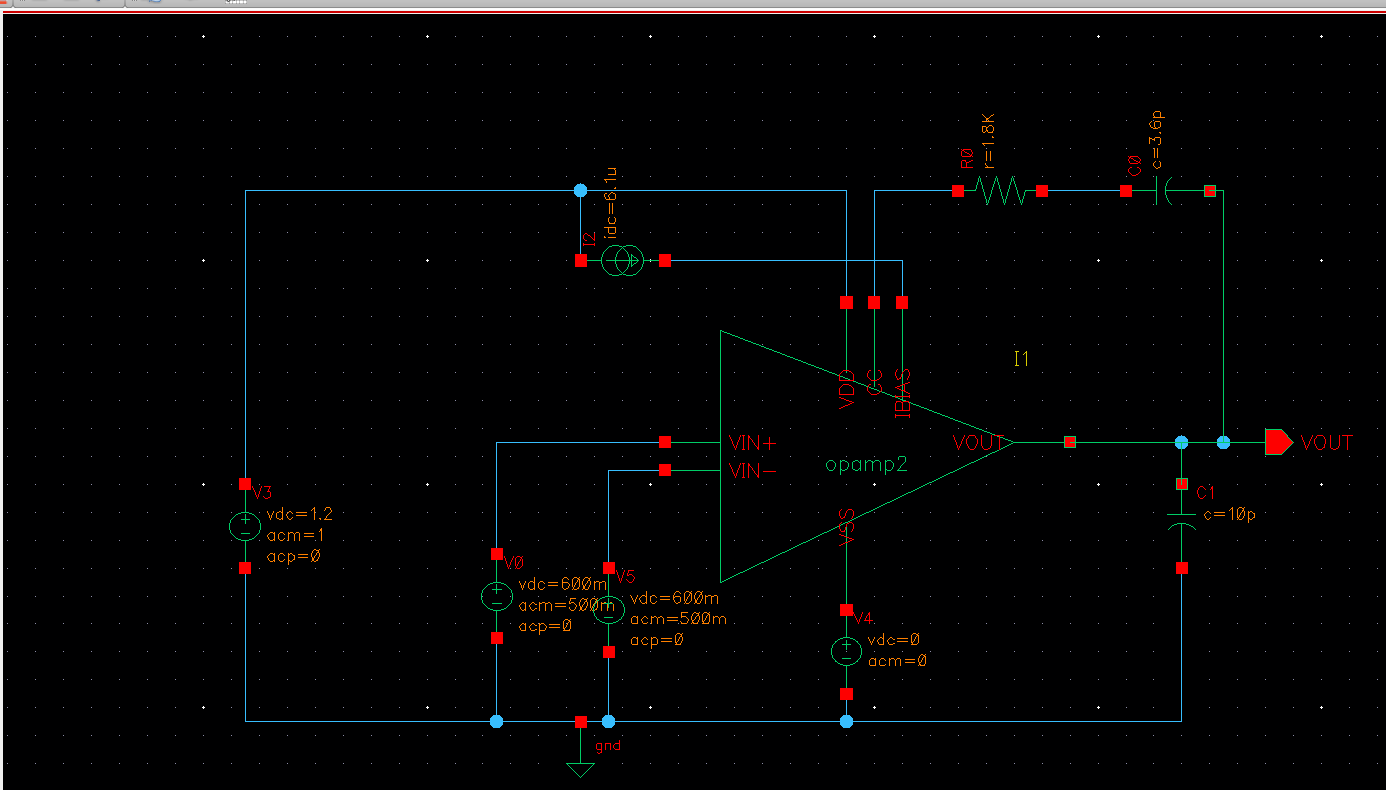
\includegraphics[width=\linewidth]{tb_psrr_plus_rz_1p8k.png}\caption{Kích AC \SI{1}{V} tại $V_{DD}$ để đo PSRR$^+$.}\end{subfigure}\hfill
\begin{subfigure}{0.48\textwidth}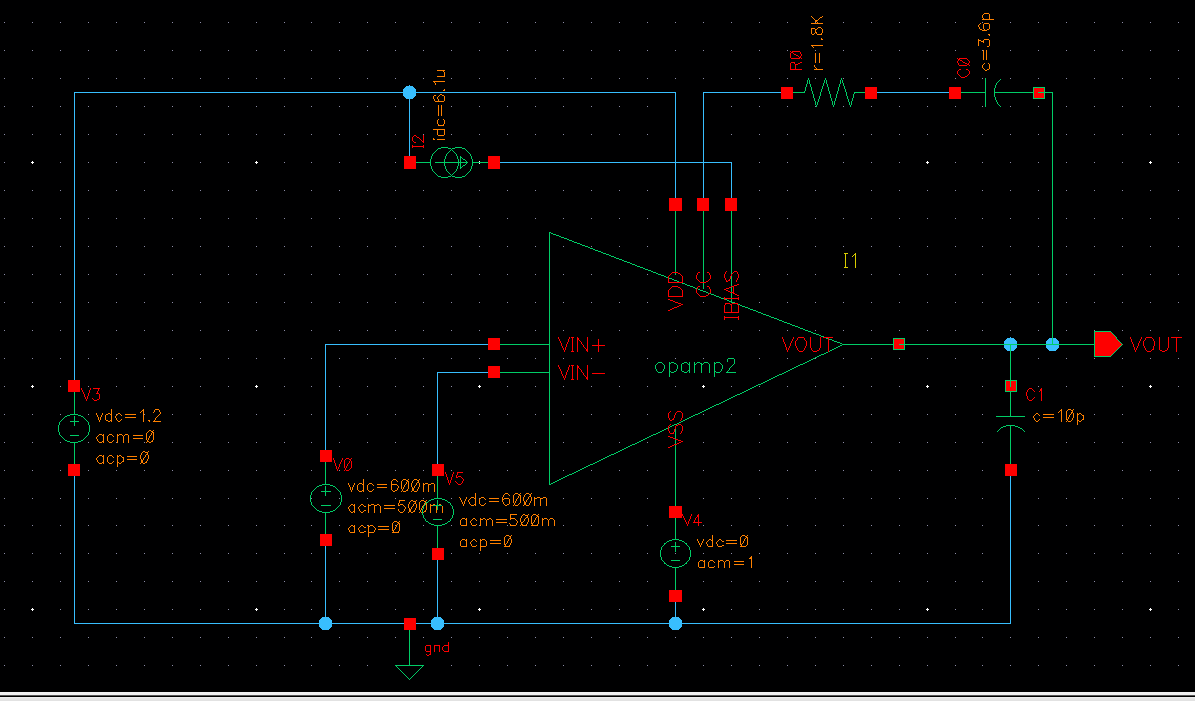
\includegraphics[width=\linewidth]{tb_psrr_minus_rz_1p8k.png}\caption{Kích AC \SI{1}{V} tại $V_{SS}$ để đo PSRR$^-$.}\end{subfigure}
\caption{Cấu hình kích nhiễu nguồn.}\end{figure}
\begin{figure}[H]\centering
\begin{subfigure}{0.49\textwidth}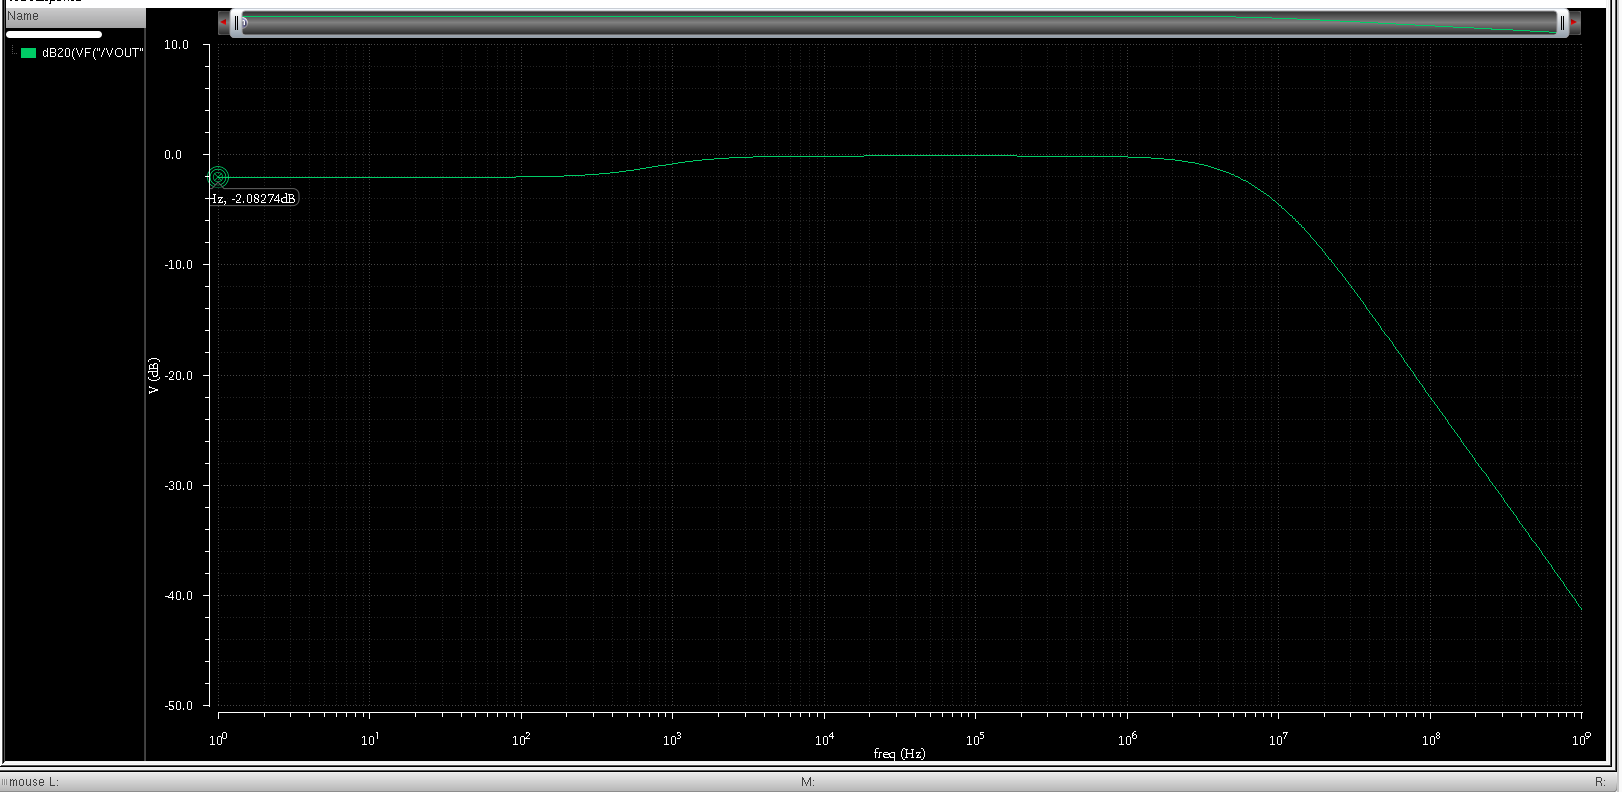
\includegraphics[width=\linewidth]{psrr_plus_rz_1p8k.png}\caption{$A_{VDD}(0)=\SI{-2.08274}{dB}$.}\end{subfigure}\hfill
\begin{subfigure}{0.49\textwidth}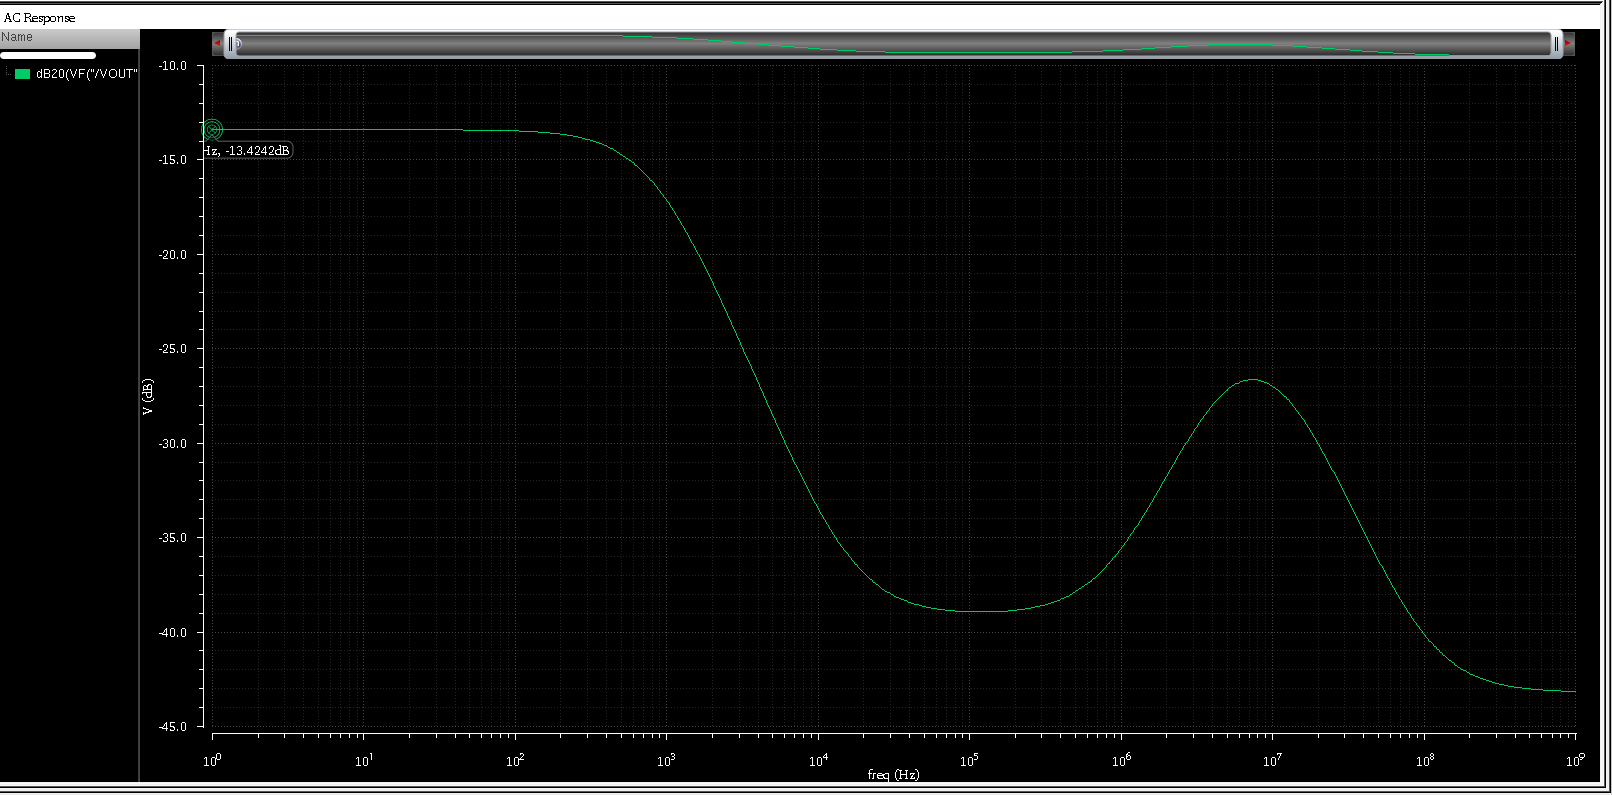
\includegraphics[width=\linewidth]{psrr_minus_rz_1p8k.png}\caption{$A_{VSS}(0)=\SI{-13.4242}{dB}$.}\end{subfigure}
\caption{Hàm truyền từ nguồn đến ngõ ra.}\end{figure}
Kết hợp các hàm truyền nguồn với độ lợi vi sai tần số thấp
$A_d(0)=\SI{74.0526}{dB}$ thu được
\begin{align}
PSRR^+(0)&=74.0526-(-2.08274)=\boxed{\SI{76.14}{dB}},\\
PSRR^-(0)&=74.0526-(-13.4242)=\boxed{\SI{87.48}{dB}}.
\end{align}
PSRR$^-$ lớn hơn PSRR$^+$ khoảng \SI{11.34}{dB} ở tần số thấp, cho thấy
nhiễu từ rail dương ghép tới ngõ ra mạnh hơn nhiễu từ rail âm trong cấu trúc
và điểm phân cực đang xét. Các giá trị trên là PSRR tần số thấp; khả năng khử
nhiễu giảm theo tần số và cần được đọc như một hàm của tần số khi đánh giá
nhiễu nguồn ngoài dải thấp.

\chapter{Phân tích transient}
\section{Đáp ứng bước voltage follower}
Op-amp được mắc voltage follower bằng cách nối trực tiếp $V_{OUT}$ về $V_{IN-}$.
Nguồn xung tại $V_{IN+}$ chuyển giữa \SI{0.4}{V} và \SI{0.8}{V}, thời gian
cạnh đặt là \SI{1}{ns}; tải ngõ ra là \SI{10}{pF}. Mạch vẫn sử dụng
$R_z=\SI{1.8}{k\ohm}$ và $C_C=\SI{3.6}{pF}$.
\figwide[0.92\textwidth]{tb_transient_rz_1p8k.png}{Testbench transient ở cấu hình voltage follower.}
\figwide[0.98\textwidth]{transient_step_rz_1p8k.png}{Đáp ứng transient với marker tại các mức 10\% và 90\% của bước \SI{0.4}{V}.}

Với bước từ \SI{0.4}{V} lên \SI{0.8}{V}, các mức 10\% và 90\% tương ứng
xấp xỉ \SI{0.44}{V} và \SI{0.76}{V}. Từ các marker trên đồ thị:
\begin{align}
t_{r,10-90}&=1.103319-1.024743
=\boxed{\SI{78.58}{ns}},\\
t_{f,90-10}&=6.117794-6.028390
=\boxed{\SI{89.40}{ns}}.
\end{align}
Đồ thị cho thấy ngõ ra bám đúng hai mức xác lập xấp xỉ \SI{0.4}{V} và
\SI{0.8}{V}, đồng thời có overshoot và undershoot nhỏ sau mỗi cạnh. Tuy nhiên,
các marker hiện tại là marker 10--90\%, không phải biên sai số 1\%; vì vậy chưa
thể dùng chúng để kết luận định lượng settling time 1\%.

\section{Slew rate}
\begin{equation}SR_{calc}=\frac{\SI{18}{\micro A}}{\SI{3.6}{pF}}=\boxed{\SI{5}{V/\micro s}}.\end{equation}
Từ độ dốc trung bình giữa hai marker 10\% và 90\% thu được
\begin{align}
SR_{+,10-90}&\approx\frac{0.7603913-0.4406157}{0.078576}
=\boxed{\SI{4.07}{V/\micro s}},\\
SR_{-,90-10}&\approx-\frac{0.7602219-0.4401017}{0.089404}
=\boxed{\SI{-3.58}{V/\micro s}}.
\end{align}
Đây là tốc độ chuyển mức trung bình trong vùng 10--90\%, không phải cực đại của
đạo hàm $\dd V_{OUT}/\dd t$. Cả hai thấp hơn giá trị first-cut
\SI{5}{V/\micro s}, phù hợp với việc một phần dòng phải nạp các điện dung nội và
tầng ngõ ra không phải nguồn dòng lý tưởng.

\chapter{Layout vật lý}
\section{Thiết kế full-custom}
Layout được bố trí theo dòng tín hiệu của schematic. Các cặp matching M1--M2 và M3--M4 cần cùng hướng, cùng môi trường xung quanh và định tuyến đối xứng. Nút trở kháng cao tầng một phải ngắn và tránh ghép với ngõ ra biên độ lớn.
\figwide[0.76\textwidth]{layout.png}{Layout full-custom của op-amp hai tầng bù Miller.}

\section{Extracted view}
\figwide[0.86\textwidth]{av_extracted.png}{Layout extracted/annotated dùng kiểm tra kết nối.}
Các hình không thay thế cho DRC, LVS và PEX. Netlist hậu layout phải được mô phỏng lại DC gain, unity frequency, phase margin, settling, slew rate, CMRR và PSRR.

\chapter{Kết quả và thảo luận}
\section{Tổng hợp thông số}
\begin{table}[H]\centering\caption{Mục tiêu và mô phỏng danh định.}
\begin{tabularx}{\textwidth}{>{\bfseries}l l l >{\raggedright\arraybackslash}X}\toprule
Chỉ tiêu&Mục tiêu&Kết quả&Đánh giá\\\midrule
Độ lợi DC&$\ge\SI{70}{dB}$&\SI{74.05}{dB}&\pass\\
Unity frequency&$\ge\SI{3}{MHz}$&$\approx\SI{3.802}{MHz}$&\pass\\
Phase margin&$\ge\ang{60}$&$\approx\ang{62.13}$&\pass\\
Băng thông pole trội&---&\SI{851.14}{Hz}&Thông tin\\
Slew rate 10--90\%&\SI{5}{V/\micro s}&$+\approx4.07$, $-\approx3.58$&\fail\\
Rise/fall time 10--90\%&---&\SI{78.58}{ns}/\SI{89.40}{ns}&Đã đo\\
Settling 1\%&$\le\SI{1}{\micro s}$&Chưa đặt marker dải 1\%&Cần đo lại\\
ICMR&\SIrange{0.4}{0.9}{V}&\SIrange{0.313}{0.936}{V}&\pass\\
Output swing&cực đại&$\approx\SIrange{0.00}{1.12}{V}$&$\approx\SI{1.12}{Vpp}$\\
CMRR&---&\SI{73.60}{dB}&Đã chuẩn hóa theo $V_{CM}=\SI{0.5}{V}$\\
PSRR$^+$ / PSRR$^-$&---&\SI{76.14}{dB}/\SI{87.48}{dB}&Kích nguồn AC \SI{1}{V}\\
Ngõ ra tĩnh&gần giữa nguồn&\SI{0.598}{V}&\pass\\
Công suất tĩnh&---&\SI{153.249}{\micro W}&Đo trực tiếp tại nguồn $V_{DD}$\\\bottomrule
\end{tabularx}\end{table}

\section{Đánh đổi chính}
Giảm $C_C$ tăng GBW và slew rate nhưng làm giảm phase margin. Tăng $g_{m1}$ tăng GBW nhưng cần tăng dòng hoặc kích thước cặp đầu vào. Tăng $g_{m6}$ cải thiện pole thứ hai nhưng tăng công suất và có thể làm zero RHP ảnh hưởng mạnh hơn. Điện trở nulling $R_z\approx1/g_{m6}\approx\SI{1.81}{k\ohm}$ có thể loại bỏ zero RHP. Kênh dài hơn tăng intrinsic gain nhưng giảm tốc độ và tăng diện tích.

\chapter{Kết luận}
Op-amp CMOS tám transistor, hai tầng, bù Miller đã được thiết kế trong GPDK090 với nguồn \SI{1.2}{V} và tải \SI{10}{pF}. Tính toán cho bộ phân cực nhất quán với $I_5=\SI{18}{\micro A}$, $S_5=11.18$ và $S_8=3.79$. Operating point xác nhận dòng vi sai cân bằng, dòng tầng ngõ ra cân bằng, các transistor bão hòa và ngõ ra tĩnh gần giữa nguồn.

Mô phỏng danh định cho \SI{74.05}{dB} gain, khoảng \SI{3.802}{MHz} unity frequency, \ang{62.13} phase margin, ICMR xấp xỉ \SIrange{0.313}{0.936}{V}, thời gian chuyển mức 10--90\% khoảng \SI{78.58}{ns}/\SI{89.40}{ns}, output swing khoảng \SI{1.12}{Vpp}, CMRR \SI{73.60}{dB}, PSRR$^+$ \SI{76.14}{dB}, PSRR$^-$ \SI{87.48}{dB} ở tần số thấp và công suất tĩnh \SI{153.249}{\micro W}. Các yêu cầu gain, unity frequency, phase margin và ICMR đều đạt; slew rate đo theo vùng 10--90\% còn thấp hơn mục tiêu \SI{5}{V/\micro s}, còn settling time 1\% cần được đo lại bằng marker đúng định nghĩa. Điện trở nulling \SI{1.8}{k\ohm} đã cải thiện phase margin trong khi mạch vẫn duy trì unity frequency cao hơn \SI{3}{MHz}.

\begin{thebibliography}{9}
\bibitem{razavi}B. Razavi, \emph{Design of Analog CMOS Integrated Circuits}, 2nd ed., McGraw-Hill, 2017.
\bibitem{baker}R. J. Baker, \emph{CMOS: Circuit Design, Layout, and Simulation}, 3rd ed., Wiley-IEEE, 2010.
\bibitem{allen}P. E. Allen, \emph{CMOS Analog Circuit Design}, Lecture 22:
``Compensation of Op Amps,'' 2016.
\bibitem{cadence}Cadence Design Systems, \emph{Virtuoso ADE and Spectre Circuit Simulator}.
\bibitem{gpdk}GPDK090 BSIM3 MOSFET models.
\end{thebibliography}

\appendix
\chapter{Định nghĩa phép đo}
\begin{align}
A_{d,dB}(f)&=20\log_{10}\left|V_{OUT}/V_{ID}\right|,\\
A_{cm,dB}(f)&=20\log_{10}\left|V_{OUT}/V_{ICM}\right|,\\
CMRR_{dB}(f)&=A_{d,dB}(f)-A_{cm,dB}(f),\\
PSRR^+_{dB}(f)&=A_{d,dB}(f)-20\log_{10}\left|V_{OUT}/V_{DD,ac}\right|,\\
PSRR^-_{dB}(f)&=A_{d,dB}(f)-20\log_{10}\left|V_{OUT}/V_{SS,ac}\right|,\\
SR_+&=\max(\dd V_{OUT}/\dd t),\qquad SR_-=\min(\dd V_{OUT}/\dd t).
\end{align}
Thời gian xác lập được đo từ thời điểm đầu vào đi qua 50\% đến lần cuối ngõ ra đi vào dải sai số mà không rời khỏi dải sau đó.
\end{document}
